\documentclass[11pt]{article}

\usepackage[margin=1in]{geometry}
\usepackage{amsmath,amssymb}
\usepackage{graphicx}
\usepackage{booktabs}
\usepackage{hyperref}
\usepackage[numbers]{natbib}

\title{Critical error rate analysis for MSA-based variant phasing\\in nanopore amplicon sequencing}
\author{Josh Walker}
\date{}

\begin{document}
\maketitle

\begin{abstract}
Amplicon consensus tools that detect intra-specimen sequence variants must
distinguish real biological variation from sequencing error. We present a
statistical framework for evaluating the significance of variants detected by
MSA-based position phasing in Oxford Nanopore amplicon data. Rather than
computing $p$-values against a fixed error rate, we derive the \emph{critical
error rate} $p^*$: the per-position sequencing error rate at which an observed
variant pattern would become plausible under a null hypothesis of independent
errors. Using conservative assumptions---total input reads as the sample
denominator and Bonferroni correction over all amplicon positions---we show that
variants with moderate read support require per-position error rates exceeding
those of current nanopore chemistry to be explained as artifacts. We present
results under both a conservative error model ($q = p$, maximally biased
substitution) and a uniform model ($q = p/3$), and examine the effect of
significance level on variant confidence across a range of operating conditions.
\end{abstract}

\section{Introduction}

Oxford Nanopore sequencing of PCR amplicons is widely used for taxonomic
identification, particularly in fungal DNA barcoding of the internal transcribed
spacer (ITS) region~\cite{schoch2012}. After demultiplexing, reads from a single
specimen are clustered and consensus sequences are generated to produce
high-accuracy reference sequences suitable for database matching.

When a specimen contains multiple sequence variants---arising from heterozygosity,
paralogous loci, mixed templates, or multi-copy rDNA polymorphism---the clustering
and consensus pipeline must resolve these into separate consensus sequences rather
than collapsing them into a single ambiguous output. Speconsense addresses this
through MSA-based variant phasing: after initial clustering, it examines the
multiple sequence alignment within each cluster to identify positions where a
substantial fraction of reads consistently differ from the consensus, then
recursively splits the cluster into haplotype groups based on allele patterns at
these positions.

A natural concern is whether detected variants represent real biological
sequences or artifacts of sequencing error. If nanopore errors at a particular
position happened to affect the same base in enough reads, the phasing algorithm
could mistake this for a genuine variant. We address this concern by deriving the
per-position error rate required to make each variant plausible as an artifact,
and showing that this critical rate exceeds realistic nanopore error for variants
with sufficient read support.

\section{Methods}

\subsection{Null model}

Under the null hypothesis, all reads in a cluster originate from a single true
sequence, and observed base differences are independent sequencing errors. At
each position, each read independently has probability $p$ of containing an
error.

We present results under two substitution models:

\begin{itemize}
\item \textbf{Conservative} ($q = p$): All errors at a position produce the same
alternative base. This represents the worst case, accounting for nanopore
substitution biases that favor certain error types~\cite{wick2023}. If errors are
concentrated toward one alternative base, the probability of multiple reads
independently producing the same incorrect base is maximized.

\item \textbf{Uniform} ($q = p/3$): Errors are spread equally across the three
alternative bases. This is more realistic for positions without strong substitution
bias, and provides a less conservative bound.
\end{itemize}

\subsection{Parameter definitions}

\begin{itemize}
\item $N$: Total input read count for the specimen, before clustering. This is
conservative because it represents the full pool from which a biased subsample
could be drawn. In practice, speconsense uniformly presamples to $N \leq 1000$
reads, so this is bounded.

\item $M$: Number of reads supporting the variant allele at a position.

\item $L$: Amplicon length in base pairs. For the ITS region, $L \approx 700$~bp.
This determines the multiple testing correction.

\item $K$: Number of variant positions distinguishing a given variant from all
other variants produced from the same specimen. The main analysis uses $K = 1$
(single-position variants), the hardest case.

\item $\alpha$: Significance level. We examine $\alpha = 0.05$ (per-variant),
$\alpha = 10^{-3}$, and $\alpha = 10^{-5}$ (appropriate when correcting for
thousands of variant calls across a sequencing run).
\end{itemize}

\subsection{Critical error rate for single-position variants ($K = 1$)}

For a single position where $M$ of $N$ reads share the same alternative base,
the probability under the null model is given by the binomial survival function:
\begin{equation}
P(\text{position is artifact}) = P\bigl(\text{Binom}(N,\, q) \geq M\bigr)
\end{equation}
where $q = p$ (conservative) or $q = p/3$ (uniform).

With Bonferroni correction over $L$ independent positions, the probability that
\emph{any} position exhibits a variant-like pattern is bounded by:
\begin{equation}
P(\text{any artifact variant}) \leq L \cdot P\bigl(\text{Binom}(N,\, q) \geq M\bigr)
\end{equation}

The critical error rate $p^*$ is defined as the value of $p$ satisfying:
\begin{equation}
\label{eq:critical}
L \cdot P\bigl(\text{Binom}(N,\, q^*) \geq M\bigr) = \alpha
\end{equation}

This is a single-variable equation solved numerically via root-finding on the
log-scale survival function. If $p^*$ substantially exceeds the actual
per-position error rate of the sequencing platform, the variant cannot plausibly
be explained by error.

\subsection{Choice of significance level}

A single variant call at $\alpha = 0.05$ has a 5\% false positive probability
under the null. In a typical sequencing run producing thousands of variant calls
across hundreds of specimens, the run-level false positive rate can be
substantial. For a run of $S$ specimens producing an average of $V$ variants
each, the expected number of false positives is $\alpha \cdot S \cdot V$.

With $S = 1000$ and $V \approx 3$, $\alpha = 0.05$ yields ${\sim}150$ expected
false positives per run. A Bonferroni correction to the run level suggests
$\alpha \approx 0.05 / 3000 \approx 1.7 \times 10^{-5}$. We therefore present
results at $\alpha = 10^{-5}$ as a practical run-corrected threshold alongside
the per-variant $\alpha = 0.05$.

\subsection{Extension to multi-position variants ($K > 1$)}

When $K$ positions independently distinguish a variant, the probability under the
null that all $K$ simultaneously exhibit the same allele pattern is:
\begin{equation}
P(\text{$K$-position artifact}) \leq \binom{L}{K} \cdot
\Bigl[P\bigl(\text{Binom}(N,\, q) \geq M\bigr)\Bigr]^K
\end{equation}

Setting this equal to $\alpha$ and solving for $p^*$ yields a per-position target:
\begin{equation}
P\bigl(\text{Binom}(N,\, q^*) \geq M\bigr) =
\left(\frac{\alpha}{\binom{L}{K}}\right)^{1/K}
\end{equation}

Although the combinatorial correction $\binom{L}{K}$ grows rapidly ($\binom{700}{2}
= 244{,}650$; $\binom{700}{3} = 57{,}085{,}400$), the $K$-th root dominates, and
the per-position target actually \emph{increases} with $K$. In practice, any
variant distinguished at $K \geq 2$ positions is at least as significant as a
single-position variant.

\section{Results}

\subsection{Critical error rates at fixed $N$}

Figure~\ref{fig:vs_M} shows the critical error rate $p^*$ as a function of
variant read count $M$ at $N = 1000$ (the standard presample size) for $K = 1$.
Curves are shown for three significance levels under the conservative model
($q = p$), with the uniform model ($q = p/3$) overlaid at $\alpha = 0.05$ and
$\alpha = 10^{-5}$ for comparison.

Under the conservative model at $\alpha = 0.05$, a variant supported by $M = 50$
reads exceeds the 5\% error rate reference line, and $M = 100$ yields
$p^* = 6.8\%$. Even at the stringent run-corrected $\alpha = 10^{-5}$, $M = 100$
gives $p^* = 5.5\%$---still well above realistic nanopore error rates. The
difference between significance levels is modest at high $M$, reflecting the
exponential sensitivity of the binomial test.

Under the uniform model, the same cases yield $p^* = 20.3\%$ and $16.6\%$
respectively, providing comfortable margins.

At low $M$ (${<}20$ reads), the critical error rate drops below 1\% under the
conservative model regardless of significance level, indicating that variants
with very few supporting reads approach the boundary of statistical
distinguishability.

\begin{figure}[htbp]
\centering
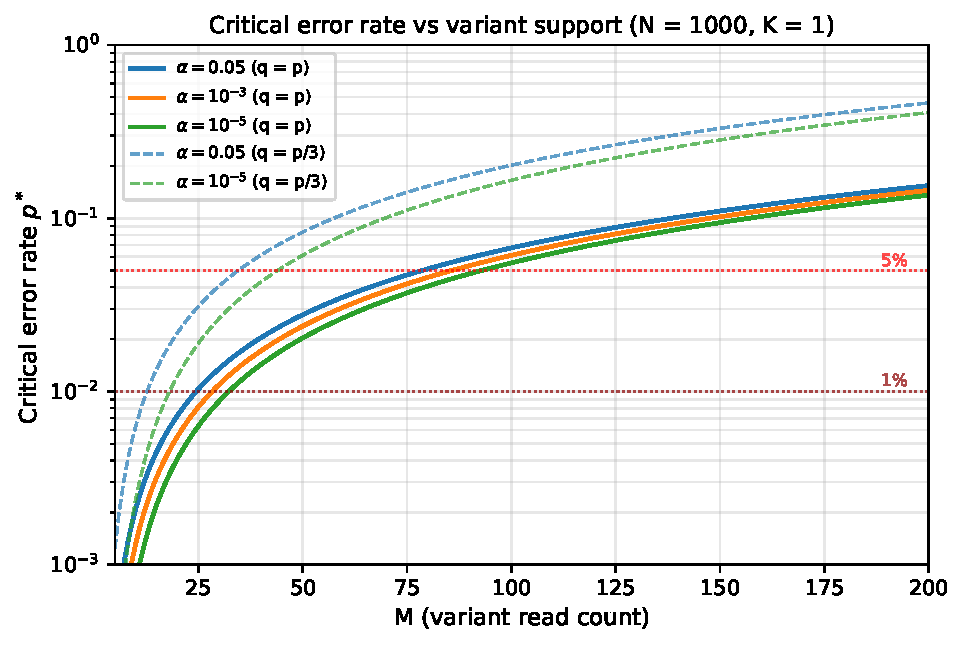
\includegraphics[width=\textwidth]{figures/fig1_critical_rate_vs_M.pdf}
\caption{Critical error rate $p^*$ vs.\ variant read count $M$ at $N = 1000$,
$K = 1$, $L = 700$. Solid lines: conservative model ($q = p$) at three
significance levels. Dashed lines: uniform model ($q = p/3$) at $\alpha = 0.05$
and $\alpha = 10^{-5}$.}
\label{fig:vs_M}
\end{figure}

\subsection{Effect of total read count}

Figure~\ref{fig:by_N} shows $p^*$ as a function of $M$ for several values of $N$
under both error models ($\alpha = 0.05$). For a given $M$, larger $N$ yields
lower $p^*$ because the same absolute count represents a smaller fraction of the
total pool.

The side-by-side comparison illustrates the roughly threefold difference between
error models. Under the uniform model, even relatively modest support ($M = 20$
at $N = 1000$) yields $p^*$ above 1\%. Under the conservative model, $M \approx
30$ is needed to reach the same threshold.

\begin{figure}[htbp]
\centering
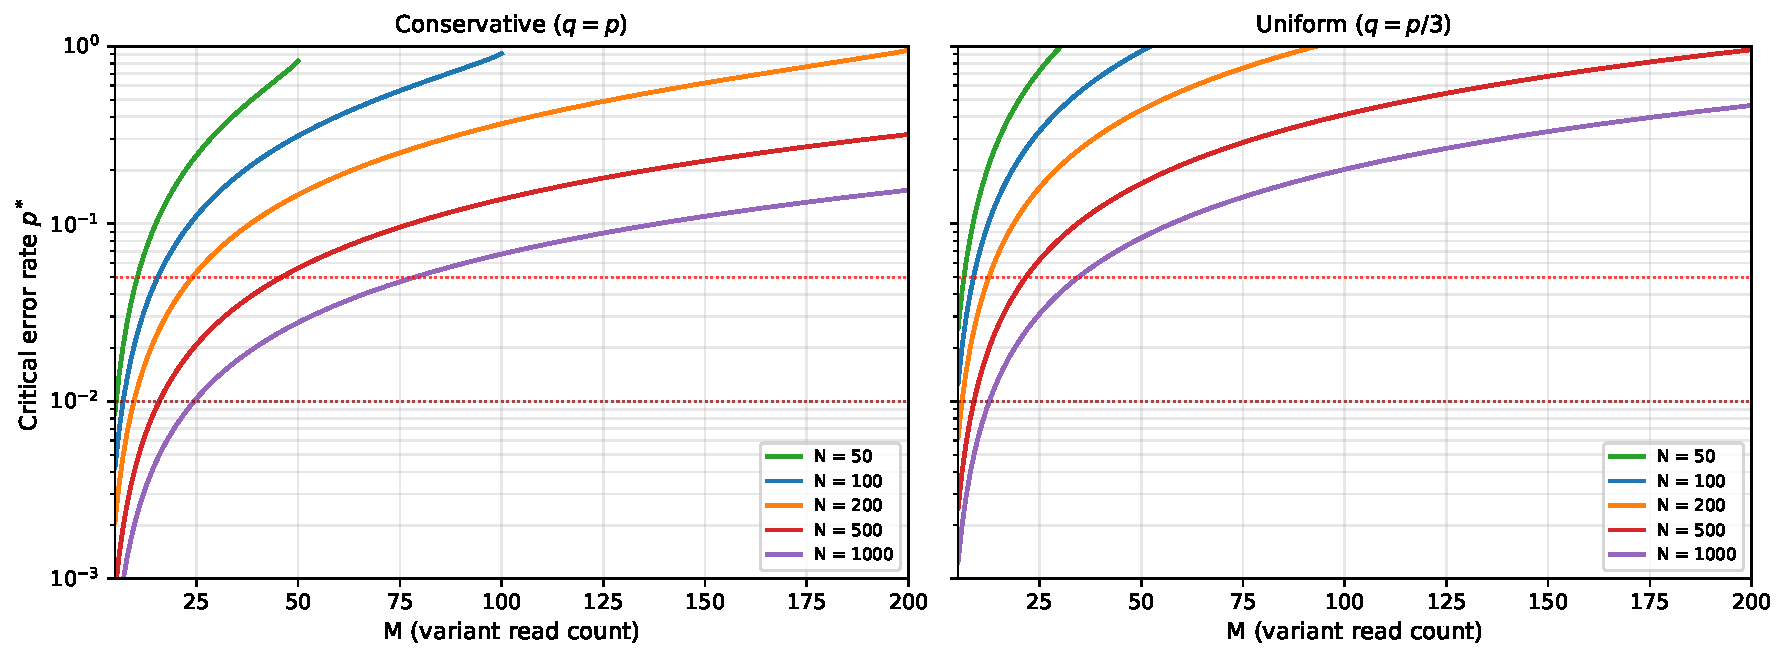
\includegraphics[width=\textwidth]{figures/fig2_critical_rate_by_N.pdf}
\caption{Critical error rate $p^*$ vs.\ variant read count $M$ for several total
read counts $N$ ($K = 1$, $L = 700$, $\alpha = 0.05$). Left: conservative model
($q = p$). Right: uniform model ($q = p/3$).}
\label{fig:by_N}
\end{figure}

\subsection{Multi-position variants}

For variants distinguished at $K \geq 2$ positions, the critical error rate
increases modestly (Appendix, Figure~\ref{fig:K_comparison}). The improvement is
small in absolute terms because the single-position binomial test is already
highly sensitive at these sample sizes. Any variant distinguished at multiple
positions is at least as well-supported as a single-position variant.

\subsection{Summary of key values}

Table~\ref{tab:key_values} summarizes critical error rates for representative
parameter combinations under both error models.

\begin{table}[htbp]
\centering
\caption{Critical error rates $p^*$ for representative parameter combinations
($K = 1$, $L = 700$). Values shown for both conservative ($q = p$) and uniform
($q = p/3$) error models.}
\label{tab:key_values}
\begin{tabular}{rrrrrr}
\toprule
 & & & \multicolumn{2}{c}{$p^*$} & \\
\cmidrule(lr){4-5}
$N$ & $M$ & $\alpha$ & $q = p$ & $q = p/3$ & Note \\
\midrule
1000 & 100 & 0.05     & 6.75\%  & 20.25\% & Standard operating point \\
1000 & 100 & $10^{-5}$ & 5.53\%  & 16.59\% & Run-corrected \\
100  & 10  & 0.05     & 2.18\%  & 6.55\%  & Moderate coverage \\
100  & 10  & $10^{-5}$ & 0.83\%  & 2.50\%  & Run-corrected, moderate coverage \\
50   & 5   & 0.05     & 0.86\%  & 2.57\%  & Boundary case \\
50   & 5   & $10^{-5}$ & 0.15\%  & 0.44\%  & Run-corrected boundary \\
\bottomrule
\end{tabular}
\end{table}

\section{Discussion}

\subsection{Interpreting the critical error rate}

The critical error rate $p^*$ represents the per-position error rate at which a
given variant pattern becomes statistically plausible as an artifact. When the
conservative model is used ($q = p$), $p^*$ can be interpreted as the rate of
maximally biased error at a single position---the worst case where all errors
produce the same incorrect base. When the uniform model is used ($q = p/3$),
$p^*$ represents the overall per-position error rate under the assumption that
errors are unbiased across alternative bases.

For Oxford Nanopore reads, per-position substitution error rates typically
range from 1--5\% for simplex reads (Q13--Q20) and below 1\% for duplex or
consensus-corrected reads. Variants with $p^*$ substantially above these ranges
are robust; variants with $p^*$ near or below these ranges warrant caution.

\subsection{Conservative framing}

Several deliberate conservatisms ensure that critical error rates represent lower
bounds on variant significance:

\begin{enumerate}
\item \textbf{Denominator choice.} Using the total input read count $N$ rather
than the cluster size assumes the worst case: the clustering algorithm could have
drawn any subset from the full pool. In practice, reads are first clustered by
sequence similarity before phasing, so the effective denominator for error-driven
patterns is the cluster size, which is smaller than $N$.

\item \textbf{Maximally biased substitution.} The conservative model ($q = p$)
assumes all errors at a position produce the same alternative base. If errors
were spread across multiple alternatives ($q = p/3$), coherent error patterns
would be less likely.

\item \textbf{Bonferroni correction.} Treating all $L$ positions as independent
tests is conservative; nearby positions in amplicon sequences are not truly
independent, so the effective number of tests is smaller than $L$.

\item \textbf{Minimum $K$.} Using the minimum number of distinguishing positions
across all variant pairs represents the weakest case. Most variants are
distinguished at multiple positions, further increasing significance.
\end{enumerate}

\subsection{Homopolymer normalization}

The variant detection algorithm includes homopolymer normalization, which
subtracts homopolymer length variation from the base composition at each position
before evaluating variant thresholds. This removes the largest source of
systematic, position-correlated nanopore error from consideration. The null model
presented here does not account for this additional filtering, making the analysis
further conservative: the effective error rate after homopolymer normalization is
lower than the raw per-position rate.

\subsection{Environmental and mixed specimens}

The analysis assumes that $N$ reads originate from sequencing a single organism,
as is typical in specimen-based amplicon barcoding. For environmental DNA samples
or specimens containing multiple organisms, the interpretation of $N$ requires
modification. When the read pool contains sequences from multiple distinct
organisms, the relevant $N$ for evaluating intra-organism variants is the number
of reads from the target organism, not the total. The upstream clustering step
partially addresses this by separating reads from different organisms into
distinct clusters, but the formal guarantee applies within the assumption that
the initial cluster contains reads from a single source.

\subsection{Limitations}

The null model assumes independence of errors across positions within a read.
While nanopore errors can exhibit local correlations (e.g., in homopolymer
regions or around specific sequence motifs), the homopolymer normalization step
addresses the primary source of such correlation. Remaining context-dependent
error biases are not modeled, but would need to affect the same specific base at
the same position across a substantial fraction of reads to create a false
variant---a scenario not consistent with known nanopore error profiles.

The analysis also does not model the possibility of PCR-induced errors during
amplification. However, PCR errors introduced early in amplification would
produce read patterns indistinguishable from real variants at this level of
analysis, and are arguably real signals in the context of the sequenced library.

\section{Conclusion}

The critical error rate framework provides a transparent basis for evaluating
confidence in detected variants. Under typical operating conditions ($N = 1000$,
$M = 100$), critical rates of 5.5--6.8\% (conservative) or 16.6--20.3\%
(uniform) are well above realistic nanopore error, even at run-corrected
significance levels. At lower coverage ($N = 100$, $M = 10$), the conservative
model yields $p^* = 0.8$--$2.2\%$, approaching the boundary of
distinguishability for lower-quality reads. The framework allows users to assess
variant confidence for any specific $(N, M)$ combination by reading directly from
the presented curves, without requiring calibration against empirical error rate
estimates.

\begin{thebibliography}{9}

\bibitem[Schoch et~al., 2012]{schoch2012}
C.~L. Schoch, K.~A. Seifert, S.~Huhndorf, V.~Robert, J.~L. Spouge, C.~A.
Levesque, W.~Chen, and Fungal Barcoding Consortium.
\newblock Nuclear ribosomal internal transcribed spacer ({ITS}) region as a
universal {DNA} barcode marker for fungi.
\newblock \emph{Proceedings of the National Academy of Sciences},
109(16):6241--6246, 2012.

\bibitem[Wick et~al., 2023]{wick2023}
R.~R. Wick, L.~M. Judd, and K.~E. Holt.
\newblock Assembling the perfect bacterial genome using {Oxford Nanopore} and
{Illumina} sequencing.
\newblock \emph{PLOS Computational Biology}, 19(3):e1010905, 2023.

\end{thebibliography}

\appendix

\section{Multi-position variant analysis}

Figure~\ref{fig:K_comparison} compares critical error rates for $K = 1, 2, 3$
variant positions at $N = 1000$. The curves are nearly coincident, confirming
that the single-position analysis ($K = 1$) represents the conservative bound
and that multi-position variants provide at least equivalent statistical support.

\begin{figure}[htbp]
\centering
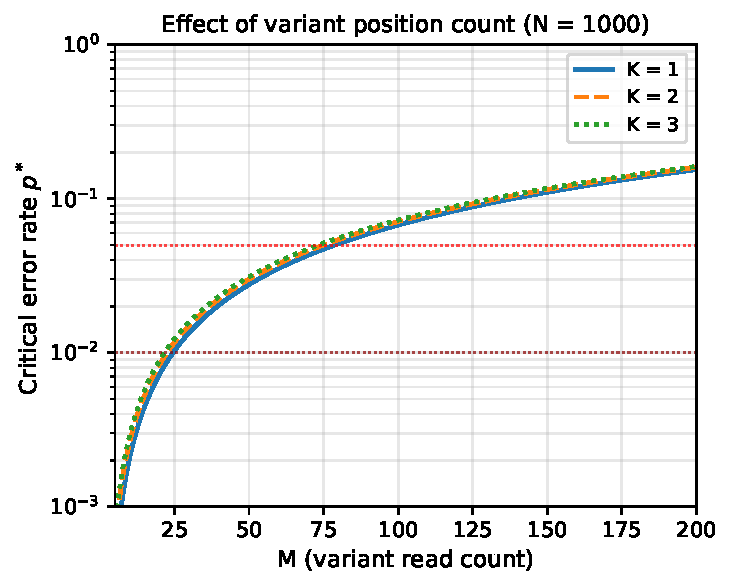
\includegraphics[width=0.7\textwidth]{figures/fig3_K_comparison.pdf}
\caption{Critical error rate $p^*$ as a function of variant read count $M$ for
$K = 1, 2, 3$ variant positions ($N = 1000$, $L = 700$, $\alpha = 0.05$,
conservative model).}
\label{fig:K_comparison}
\end{figure}

\end{document}
